\documentclass[12pt]{article}
\usepackage[
  top=2.50cm,
  bottom=1.50cm,
  left=1.50cm,
  right=1.50cm
]{geometry} 
\usepackage{amsmath,amsthm,amssymb}
\usepackage{algorithm,algorithmic}
\usepackage{graphicx}
\usepackage{tikz}

\newenvironment{theorem}[2][Theorem]{\begin{trivlist}
\item[\hskip \labelsep {\bfseries #1}\hskip \labelsep {\bfseries #2.}]}{\end{trivlist}}
\newenvironment{lemma}[2][Lemma]{\begin{trivlist}
\item[\hskip \labelsep {\bfseries #1}\hskip \labelsep {\bfseries #2.}]}{\end{trivlist}}
\newenvironment{exercise}[2][Exercise]{\begin{trivlist}
\item[\hskip \labelsep {\bfseries #1}\hskip \labelsep {\bfseries #2.}]}{\end{trivlist}}
\newenvironment{problem}[2][Problem]{\begin{trivlist}
\item[\hskip \labelsep {\bfseries #1}\hskip \labelsep {\bfseries #2.}]}{\end{trivlist}}
\newenvironment{question}[2][Question]{\begin{trivlist}
\item[\hskip \labelsep {\bfseries #1}\hskip \labelsep {\bfseries #2.}]}{\end{trivlist}}
\newenvironment{corollary}[2][Corollary]{\begin{trivlist}
\item[\hskip \labelsep {\bfseries #1}\hskip \labelsep {\bfseries #2.}]}{\end{trivlist}}

\begin{document}

\title{Homework 8}
\author{Thomas Kim~tsk389~51835\\David Munoz~dam2989~51840\\
CS331 Algorithms and Complexity}

\renewcommand{\arraystretch}{2.0}

\date{} % Suppress the datn{minipage}{0.5\textwidth}

% ------------------
% Begin Cover Page
% ------------------

\maketitle
% ------------------
% Begin Homework
% ------------------

\onecolumn

\begin{problem}
    {Q1: 13.2}
    Consider a county in which 100,000 people vote in an election.
    There are only two candidates on the ballot: a Democratic candidate (denoted $D$) and
    and Republican candidate $R$. As it happens, this county is heavily Democratic, so 80,000
    people go to the polls with the intention of voting for $D$, and 20,000 go to the polls with the intention of voting for $R$.\\

    However, the layout of the ballot is a little confusing, so each voter, independently and with probability $\frac{1}{100}$, votes for the
    wrong candidate - that is, the one that he or she \textit{didn't} intend to vote for.
    (Remember that in this election, there are only two candidates on the ballot.)\\

    Let $X$ denote the random variable equal to the number of votes received by the Democratic candidate $D$ when the voting is conducted with this
    process of error. Determine the expected value of $X$, and give an explanation of your derivation of this value.
\end{problem}

\begin{problem}
  {Q2(a)}
  Show that it is always possible to guess a number between 1 and 1 million using 20 questions.
  \begin{proof}
    TODO\\
  \end{proof}
\end{problem}

\begin{problem}
  {Q2(b)}
  Solve the same problem, but this time assume you have a limited supply $p_i$ of each coin $c_i$
  Provide a dynamic programming algorithm, do not prove correctness or runtime.
\end{problem}

\begin{problem}
  {Q2(c)}
  Assume $C = 1, 2, 4, \dots, 2^m$ and $N < 2^{m+1}$. For this special case, give an $O(m)$ time algorithm that solves the problem in (a). \\
  \begin{algorithmic}[1]
    \STATE $count = 0$
    \STATE Express $N$ as a binary number $n_1n_2n_3\dots n_k$
    \FOR {$1 \leq i \leq 2^m$}
    \IF {$n_i = 1$}
    \STATE $count := count + 1$
    \ENDIF
    \ENDFOR
  \end{algorithmic}
  \noindent
  \textbf{Correctness}
  \begin{proof}
      Thm: For every element $x \in Q_p$, where $Q_p$ is a field of $p-adic$ integers,
      there exists a unique representation $x = \sum_{i = 0}^{k} a_ip^i, a_k \neq 0$ \\
      By expressing $N$ as a 2-adic integer, it is guaranteed that there exists some
      representation of $N$ in the form shown above. \\
      Note that $k$ in the above sum is bounded by $k < m+1$, since $2^{m+1} > N$ \\
      $\forall 0 \leq i \leq m, 2^i \in C$
      Therefore, there exists a unique representation of $N$ as a sum of the elements in $C$.
  \end{proof}
  \noindent
  \textbf{Runtime}
  \begin{proof}
      Expressing $N$ as a binary number is $O(m)$ time, since $N$ expressed in binary has at most $m$ digits. \\
      Counting the $1$'s in the binary representation of $N$ takes $O(m)$ time, for the above reason.\\
      The complexity is therefore $O(2m) = O(m)$
  \end{proof}
\end{problem}

\begin{problem}
  {Q3(a)}
  ~\\
  \begin{center}
    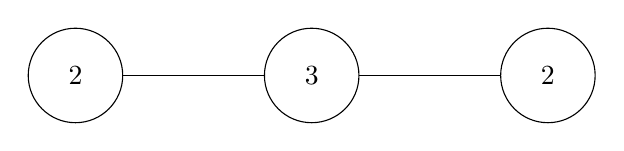
\begin{tikzpicture}[scale=0.2]
      \tikzstyle{every node}+=[inner sep=0pt]
      \draw [black] (5,0) circle (3);
      \draw (5,0) node {$2$};
      \draw [black] (20,0) circle (3);
      \draw (20,0) node {$3$};
      \draw [black] (35,0) circle (3);
      \draw [black] (35,0) node {$2$};
      \draw [black] (23,0) -- (32,0);
      \draw [black] (8,0) -- (17,0);
    \end{tikzpicture}
  \end{center}
  In this example, the middle node will be chosen and the two side nodes discarded for a total weight of $3$. \\
  If the middle node was discarded and the two side nodes chosen, the total weight would have been $4 > 3$. \\
\end{problem}

\begin{problem}
  {Q3(b)}
  ~\\
  \begin{center}
    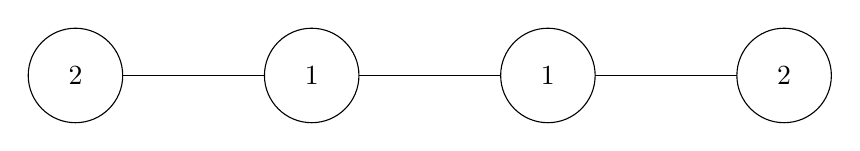
\begin{tikzpicture}[scale=0.2]
      \tikzstyle{every node}+=[inner sep=0pt]
      \draw [black] (5,0) circle (3);
      \draw (5,0) node {$2$};
      \draw [black] (20,0) circle (3);
      \draw (20,0) node {$1$};
      \draw [black] (35,0) circle (3);
      \draw (35,0) node {$1$};
      \draw [black] (50,0) circle (3);
      \draw (50,0) node {$2$};
      \draw [black] (8,0) -- (17,0);
      \draw [black] (23,0) -- (32,0);
      \draw [black] (38,0) -- (47,0);
    \end{tikzpicture}
  \end{center}
  In this example, the maximum weight independent set includes nodes $v_1$ and $v_4$, but $1$ is odd and $4$ is even. \\
\end{problem}

\begin{problem}
  {Q4} Express the $n+1$ person ballroom murder problem as a graph problem and provide an efficient way to detect inconsistencies \\
  \textbf{Graph construction algorithm}
  \begin{algorithmic}[1]
    \STATE Let $P$ be the set of people
    \STATE Let $D$ be the set of statements of the form "$i$ danced with $j$"
    \STATE Let $L$ be the set of statements of the form "$i$ saw $j$ leaving"
    \STATE Let $E$ be the set of statements of the form "$i$ saw $j$ entering"
    \STATE Let $G_1, G_2, G_3$ be empty graphs
    \FOR {$p \in P$}
    \STATE Add $p$ to $G_1, G_2, G_3$ as a vertex $v_{1,1}$ and $v_{2,1}$ respectively
    \ENDFOR
    \FOR {$l \in L$}
    \STATE Add a directed edge between $v_{1, i}$ and $v_{1, j}$
    \ENDFOR
    \FOR {$l \in E$}
    \STATE Add a directed edge between $v_{2, i}$ and $v_{2, j}$
    \ENDFOR
    \FOR {$d \in D$}
    \STATE Add a directed edge between $v_{3, i}$ and $v_{3, j}$
    \ENDFOR
  \end{algorithmic}
  \textbf{Inconsistency detection algorithm}
  \begin{algorithmic}[1]
    \STATE $T_1, T_2 = \emptyset$
    \WHILE {$\exists s \in G_1, s$ has not been explored yet}
    \STATE Perform BFS on $G_1$ starting on $s$ to generate subtree $t_{1, k}$
    \STATE $T_1 = T_1 \cup \{t_{1, k}\}$
    \ENDWHILE
    \WHILE {$\exists s \in G_2, s$ has not been explored yet}
    \STATE Perform BFS on $G_2$ starting on $s$ to generate subtree $t_{2, k}$
    \STATE $T_2 = T_2 \cup \{t_{2, k}\}$
    \ENDWHILE
    \STATE Use BFS to check for cycles in $G_1, G_2$
    \IF {$\exists$ cycle in $G_1$ or $G_2$}
    \STATE Inconsistency
    \ENDIF
    \FOR {$\forall v \in G_1$}
    \STATE Ensure all outgoing edges $e$ from $v$ in $G_3$ do not correspond to an edge between adjacent levels in any $t_{i, k} \in T_1, T_2$
    \STATE Remove $e$ from $G_3$
    \ENDFOR
  \end{algorithmic}
  \textbf{Inconsistency 1: } Odd length cycles in $G_1$ or $G_2$ imply inconsistencies with the population occupying the room. \\
  \begin{proof}
    Suppose there is a cycle in $G_1$ or $G_2$. \\
    This means $\exists p_1, p_2, \dots, p_n \in G \mid| p_x$ entered after $p_{x+1}$ left $\land p_{n} $ entered after $p_1$ left \\
    $\implies p_1$ entered after $p_k$ left, $k > 1$, particularly $p_1$ entered after $p_n$ left. \\
    This is inconsistent, as $p_1$ cannot have entered after $p_n$ left and $p_n$ entered after $p_1$ left, as each person entered the ballroom only once. \\
  \end{proof}
  \textbf{Inconsistency 2: } Edges present in $G_3$ which connect nodes in different layers of $T_1$ or $T_2$ imply inconsistency. \\
  \begin{proof}
    Suppose the graphs $G_1, G_2$ are acyclic. If they had cycles, there is already an inconsistency. \\
    Suppose two nodes are in different layers of $G_1$ or $G_2$ \\
    This means these two nodes could not have been in the room at the same time, since a parent cannot be in the same room as any child in its subtree. \\
    Suppose there is an edge present in $G_3$ which connected nodes in different layers of $T_1$ or $T_2$. \\
    This means two people who were never in the same room at the same time danced together, which is impossible. \\
  \end{proof}
  \textbf{Proof of runtime: }
  \begin{proof}
    Let the number of statements be $a$ \\
    The graph construction constructs three graphs each with $n+1$ nodes. \\
    The graph iterates through each statement once, creating $a$ edges. \\
    Therefore the number of operations taken to construct the graph is $O(3n + a + 3)$ \\
    The inconsistency detection algorithm performs BFS twice, which is $O(2m + 2n) = O(2n + 2 + 2a)$ \\
    The inconsistency detection algorithm checks for cycles during BFS by checking for any non-tree edges, which does not contribute to the complexity. \\
    The inconsistency detection algorithm then iterates through each vertex in $T_1, T_2$ and each node/edge in $G_3$, taking $O(3n + 3 + a)$ \\
    The final complexity is $O(3n + a + 3 + 2n + 2 + 2a + 3n + 3 + a) = O(8n + 4a + 8)$, which is linear complexity. \\
  \end{proof}
\end{problem}


% -----------------
% End Homework
% -----------------

\end{document}
